\documentclass[14pt,a4paper,report]{report}
\usepackage[a4paper, mag=1000, left=2.5cm, right=1cm, top=2cm, bottom=2cm, headsep=0.7cm, footskip=1cm]{geometry}
\usepackage[utf8]{inputenc}
\usepackage[english,russian]{babel}
\usepackage{indentfirst}
\usepackage[dvipsnames]{xcolor}
\usepackage[colorlinks]{hyperref}
\usepackage{listings} 
\usepackage{fancyhdr}
\usepackage{caption}
\usepackage{amsmath}
\usepackage{latexsym}
\usepackage{graphicx}
\usepackage{amsmath}
\usepackage{booktabs}
\usepackage{array}
\hypersetup{
	colorlinks = true,
	linkcolor  = black
}

\usepackage{titlesec}
\titleformat{\chapter}
{\Large\bfseries} % format
{}                % label
{0pt}             % sep
{\huge}           % before-code


\DeclareCaptionFont{white}{\color{white}} 

% Listing description
\usepackage{listings} 
\DeclareCaptionFormat{listing}{\colorbox{gray}{\parbox{\textwidth}{#1#2#3}}}
\captionsetup[lstlisting]{format=listing,labelfont=white,textfont=white}
\lstset{ 
	% Listing settings
	inputencoding = utf8,			
	extendedchars = \true, 
	keepspaces = true, 			  	 % Поддержка кириллицы и пробелов в комментариях
	language = Matlab,            	 	 % Язык программирования (для подсветки)
	basicstyle = \small\sffamily, 	 % Размер и начертание шрифта для подсветки кода
	numbers = left,               	 % Где поставить нумерацию строк (слева\справа)
	numberstyle = \tiny,          	 % Размер шрифта для номеров строк
	stepnumber = 1,               	 % Размер шага между двумя номерами строк
	numbersep = 5pt,              	 % Как далеко отстоят номера строк от подсвечиваемого кода
	backgroundcolor = \color{white}, % Цвет фона подсветки - используем \usepackage{color}
	showspaces = false,           	 % Показывать или нет пробелы специальными отступами
	showstringspaces = false,    	 % Показывать или нет пробелы в строках
	showtabs = false,           	 % Показывать или нет табуляцию в строках
	frame = single,              	 % Рисовать рамку вокруг кода
	tabsize = 2,                  	 % Размер табуляции по умолчанию равен 2 пробелам
	captionpos = t,             	 % Позиция заголовка вверху [t] или внизу [b] 
	breaklines = true,           	 % Автоматически переносить строки (да\нет)
	breakatwhitespace = false,   	 % Переносить строки только если есть пробел
	escapeinside = {\%*}{*)}      	 % Если нужно добавить комментарии в коде
}

\begin{document}

\def\contentsname{Содержание}

% Titlepage
\begin{titlepage}
	\begin{center}
		\textsc{Санкт-Петербургский Политехнический 
			Университет Петра Великого\\[5mm]
			Кафедра компьютерных систем и программных технологий}
		
		\vfill
		
		\textbf{Отчёт по лабораторной работе №4\\[3mm]
			Курс: «Методы оптимизации и принятия решений»\\[3mm]
			Тема: «Анализ GERT-сети»\\[35mm]
			}
	\end{center}
	
	\hfill
	\begin{minipage}{.5\textwidth}
		Выполнил студент:\\[2mm] 
		Ерниязов Тимур Ертлеуевич\\
		Группа: 13541/2\\[5mm]
		
		Проверил:\\[2mm] 
		Сиднев Александр Георгиевич
	\end{minipage}
	\vfill
	\begin{center}
		Санкт-Петербург\\ \the\year\ г.
	\end{center}
\end{titlepage}

% Contents
\tableofcontents
\clearpage

\chapter{Лабораторная работа №4}

\section{Задание}

\begin{figure}[h!]
	\centering
	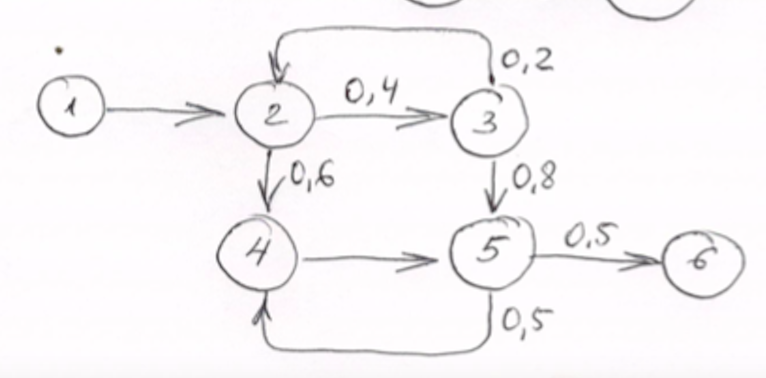
\includegraphics[scale = 0.55]{images/0.png}
	\caption{Исходный граф системы}
	\label{image:0}
\end{figure}

\subsubsection{Часть 1}

Каждой дуге ($ij$) поставлены в соответствие следующие данные:

\begin{itemize}
	\item закон распределения времени выполнения работы (будем считать его нормальным);
	\item параметры закона распределения; (математическое ожидание $M$ и дисперсия $D$).
	\item вероятность $P_{ij}$ выполнения работы, показанная на графе.
\end{itemize}

Необходимо найти:

\begin{itemize}
	\item вероятность выхода в завершающий узел графа (для всех вариантов узел 6);
	\item математическое ожидание;
	\item дисперсию времени выхода процесса в завершающий узел графа;
		\item начальные моменты первых 10 порядков.
\end{itemize}

В отчете перечислить все петли всех порядков, обнаруженные на графе, выписать уравнение Мейсона, получить решение для $W_E(s)$ и найти требуемые параметры.

\subsubsection{Часть 2}

Решить задачу используя методику анализа потокового графа, основанную на обработке матрицы передач (Branch Transmittance Matrix).

\clearpage

\section{Ход работы}

\subsection{Построение замкнутой GERT-сети}

Чтобы определить эквивалентную W-функцию для анализируемой GERT-сети, необходимо замкнуть сеть дугой, исходящей из узла 6 в узел 1:

\begin{figure}[h!]
	\centering
	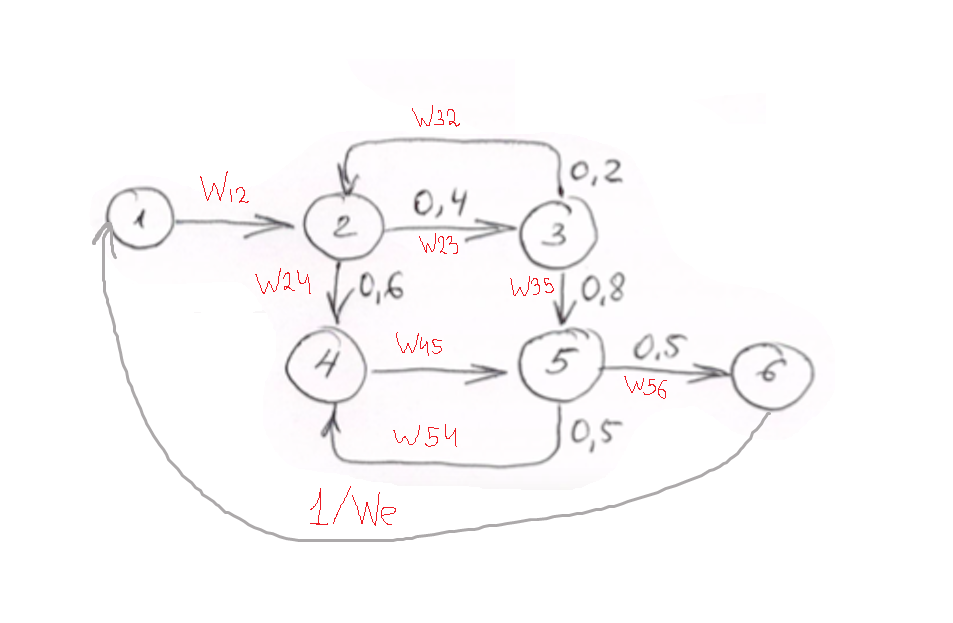
\includegraphics[scale = 0.65]{images/1.png}
	\caption{Замкнутая GERT-сеть}
	\label{image:1}
\end{figure}

\subsection{Построение W-функции}

Найдем W-функции для дуг GERT-сети:

\begin{table}[h!]
	\bgroup
	\def\arraystretch{1}
	\begin{tabular}{ | m{1.5cm} | m{1.5cm} | m{2.0cm} | m{1.0cm} | m{1.0cm} | m{3.0cm} | }
		\hline
		Начало & Конец & Вероятность & M & D & W-функция \\ \hline
		1 &  2 & 1 		& 44 & 25 & $1\cdot e^{44s+12.5s^2}$ \\ \hline
		2 & 3 & 0.4  & 24 & 25 & $0.4\cdot e^{24s+12.5s^2}$ \\ \hline
		2 & 4 & 0.6 	& 40 & 25 & $0.6\cdot e^{40s+12.5s^2}$ \\ \hline
		3 & 2 & 0.2 	& 34 & 25 & $0.2\cdot e^{34s+12.5s^2}$ \\ \hline
		3 & 5 & 0.8 	& 15 & 9 & $0.8\cdot e^{15t+4.5s^2}$ \\ \hline
		4 & 5 & 1 		& 32 & 25 & $1\cdot e^{32s+12.5s^2}$ \\ \hline
		5 & 4 & 0.5 	& 11 & 4 & $0.5\cdot e^{11s+2s^2}$ \\ \hline
		5 & 6 & 0.5 	& 24 & 25 & $0.5\cdot e^{24s+12.5s^2}$ \\ \hline
	\end{tabular}
	\egroup
\end{table}

\subsection{Построение уравнения Мейсона}

Петли первого порядка:

$W_{45}\cdot W_{54}$

$W_{23}\cdot W_{32}$

$W_{12}\cdot W_{23}\cdot W_{35}\cdot W_{56}\frac{1}{W_E}$

$W_{12}\cdot W_{24}\cdot W_{45}\cdot W_{56}\frac{1}{W_E}$

Петли второго порядка:
$W_{23}\cdot W_{32}\cdot W_{45}\cdot W_{54}$

Таким образом уравнение Мейсона будет иметь следующий вид:

$H=1 - W_{45}W_{54}-W_{23}W_{32}-W_{12}W_{23}W_{35}W_{56}\frac{1}{W_E}-W_{12}W_{24}W_{45}W_{56}\frac{1}{W_E}+W_{23}W_{32}W_{45}W_{54}$\\

В результате эквивалентная W-функция равняется:

$W_E(s)=- \frac{W_{12}W_{24}W_{45} + W_{12}W_{23}W_{34}W_{45}W_{56}}{W_{12}W_{23}W_{31} +W_{12}W_{24}W_{45}W_{53}W_{31}+W_{34}W_{45}W_{53} -1}$\\

\subsection{Рассчет статистических значений}

Расчет математического ожидания ($\mu_{1E}$) и дисперсии ($\sigma_E$) производится по следующим образом:

$W_E(s)=p_E\cdot M_E(s), p_E=W_E(0)\Longrightarrow M_E(s)=\frac{W_E(s)}{W_E(0)}$

$\mu_{1E}=\frac{d M_E(s)}{ds}|s=0$

$\mu_{2E}=\frac{d^2 M_E(s)}{ds^2}|s=0$

$\sigma_E=\mu_{2E}-\mu_{1E}^2$\\

Разработаем скрипт для расчета статистических значений в среде MATLAB:
\begin{lstlisting}[language={matlab}, caption={Matlab скрипт}, basicstyle=\ttfamily]
clear all;
close all; 
clc;
format long g;

syms s;

% W-functions
W12 = 0.5 * exp(10*s + 8 * s^2);
W16 = 0.5 * exp(23 * s + 312.5 * s^2);
W22 = 0.2 * exp(13 * s + 128 * s^2);
W26 = 0.8 * exp(11 * s + 128 * s^2);
W35 = 1 * exp(10 * s + 40.5 * s^2);
W41 = 0.4 * exp(37 * s + 128 * s^2);
W43 = 0.3 * exp(12 * s + 128 * s^2);
W46 = 0.3 * exp(12 * s + 1200.5 * s^2);
W54 = 0.3 * exp(15 * s + 312.5  * s^2);
W55 = 0.5 * exp(19 * s + 8 * s^2);
W56 = 0.2 * exp(42 * s + 40.5 * s^2);

% We(s)
We = (W12 * W26 + W16 - W16 * W22 - W16 * W35 * W54 * W43 - W16 * W55 - W12 * W26 * W55 - W12 * W26 * W35 * W54 * W43 + W16 * W22 * W35 * W54 * W43 + W16 * W22 * W55) / (1 - W35 * W54 * W43 - W22 - W55 + W22 * W55 + W22 * W35 * W54 * W43);
We = simplify(We);

% We(0)
We0 = subs(We, 's', 0);
fprintf('We(0) = %.3f\n', double(We0));

% Me(s)
Me = We / We0;

% me1
me1 = diff(Me, 's', 1);
me1 = subs(me1, 's', 0);
fprintf('me1 = %.3f\n', double(me1));

% me2
me2 = diff(Me, 's', 2);
me2 = subs(me2, 's', 0);
fprintf('me2 = %.3f\n', double(me2));

% de
de = me2 - me1 ^ 2;
fprintf('de = %.3f\n', double(de));

\end{lstlisting}


Результат вычисления статистических значений:

\begin{lstlisting}[language={matlab}, caption={Matlab скрипт}, basicstyle=\ttfamily]
We(0) = 1.000
me1 = 23.625
me2 = 1065.438
de = 507.297
\end{lstlisting}


\subsection{Часть 2}

Определим матрицу Q:
\begin{equation*}
Q = 
 \begin{pmatrix}
  0 & q_{12} & 0 & 0 & 0 & 0 \\
  0 & 0 & q_{23} & q_{24} & 0 & 0 \\ 
  q_{31} & 0 & 0 & q_{34} & 0 & 0 \\ 
  0 & 0 & 0 & 0 & q_{45} & q_{46} \\ 
  0 & 0 & q_{53} & 0 & 0 & q_{56} \\ 
  w_{61} & 0 & 0 & 0 & 0 & 0 
 \end{pmatrix}
\end{equation*}
Определим матрицу коэффициентов $A=I_6-Q^T$.
\begin{equation*}
A = 
 \begin{pmatrix}
    1&       0&    -q_{31}&    0&    0& -w_{61}\\
 -q_{12}& 1 & 0&    0&       0&    0\\
    0&    -q_{23}&    1&    0&       -q_{53}&    0\\
    0&       -q_{24}& -q_{34}&    1&       0&    0\\
    0&       0&    0& -q_{45}& 1 &    0\\
    0&       0&    0&    -q_{46}&    -q_{56}&    1
 \end{pmatrix}
\end{equation*}
Находим 
\begin{equation*}
det(A)
\end{equation*}
далее
\begin{equation*}
\frac{\partial det(A)}{\partial w_{61}}
\end{equation*}
\begin{equation*}
det(A | w_{61}=0)
\end{equation*}
Далее можно вывести $W_E(S)$ с помощью формулы:
\begin{equation*}
W_E(S)=-\frac{\frac{\partial det(A)}{\partial w_{61}}}{det(A | w_{61}=0)}
\end{equation*}
Для расчетов, был написан matlab скрипт.
\begin{lstlisting}[language={matlab}, caption={Matlab скрипт}, basicstyle=\ttfamily]
clc; clearvars

syms q12
syms q22
syms q23
syms q32
syms q34
syms q45
syms q51
syms q55
syms q56
syms w61
syms s

Q=[0 q12 0 0 0 0;
   0 q22 q23 0 0 0;
   0 q32 0 q34 0 0;
   0 0 0 0 q45 0;
   q51 0 0 0 q55 q56;
   w61 0 0 0 0 0];

A1 = eye(size(Q,1)) - transpose(Q);
disp(A1);

det_A1 = det(A1);

det_dw=diff(det_A1, w61);

det2_A1=subs(det_A1, w61, 0);

We= -det_dw/det2_A1;
disp(We);
\end{lstlisting}

\begin{lstlisting}[language={matlab}, caption={Результат}, basicstyle=\ttfamily]
[    1,       0,    0,    0,    -q51, -w61]
[ -q12, 1 - q22, -q32,    0,       0,    0]
[    0,    -q23,    1,    0,       0,    0]
[    0,       0, -q34,    1,       0,    0]
[    0,       0,    0, -q45, 1 - q55,    0]
[    0,       0,    0,    0,    -q56,    1]
 
 
-(q12*q23*q34*q45*q56)/(q22 + q55 + q23*q32 - q22*q55 - q23*q32*q55 + q12*q23*q34*q45*q51 - 1)
\end{lstlisting}
Во второй строчке был получен $W_E(S)$, который полностью(за исключением знаков) совпадает с $W_E(S)$ найденным в части 1.

Далее, имея $W_E(S)$ находим необходимые переменные.
\begin{lstlisting}[language={matlab}, caption={Matlab скрипт}]
clc; clearvars

%М — математическое ожидание
%D — дисперсия
%P — вероятность
P12 = 1; M12 = 20; D12 = 9; 
P22 = 0.6; M22 = 30; D22 = 16; 
P23 = 0.4; M23 = 40; D23 = 25; 
P32 = 0.5; M32 = 28; D32 = 16; 
P34 = 0.5; M34 = 37; D34 = 16; 
P45 = 1; M45 = 30; D45 = 25; 
P51 = 0.2; M51 = 30; D51 = 16; 
P55 = 0.1; M55 = 10; D55 = 4; 
P56 = 0.7; M56 = 30; D56 = 16; 

syms q12
syms q22
syms q23
syms q32
syms q34
syms q45
syms q51
syms q55
syms q56
syms w61
syms s

Q=[0 q12 0 0 0 0;
   0 q22 q23 0 0 0;
   0 q32 0 q34 0 0;
   0 0 0 0 q45 0;
   q51 0 0 0 q55 q56;
   w61 0 0 0 0 0];

A1 = eye(size(Q,1)) - transpose(Q);
disp(A1);

det_A1 = det(A1);
disp(det_A1);

det_dw=diff(det_A1, w61);
disp(det_dw);

det2_A1=subs(det_A1, w61, 0);
disp(det2_A1);

We= -det_dw/det2_A1;
disp(We);


syms s

We=subs(We, q12, P12*exp(M12*s+D12/2*s^2));
We=subs(We, q22, P22*exp(M22*s+D22/2*s^2));
We=subs(We, q23, P23*exp(M23*s+D23/2*s^2));
We=subs(We, q32, P32*exp(M32*s+D32/2*s^2));
We=subs(We, q34, P34*exp(M34*s+D34/2*s^2));
We=subs(We, q45, P45*exp(M45*s+D45/2*s^2));
We=subs(We, q51, P51*exp(M51*s+D51/2*s^2));
We=subs(We, q55, P55*exp(M55*s+D55/2*s^2));
We=subs(We, q56, P56*exp(M56*s+D56/2*s^2));

We = simplify(We)
We0 = subs(We, 's', 0)  % We(0)
 
% Нахождение мат. ожидания и дисперсии
Me = We/We0;
 
% Нахождение производной 1-го порядка при s=0
m1 = diff(Me, 's');     
m1 = subs(m1, 's', 0)   % Замена символа s на 0 в выражении m1
 
% Нахождение производной 2-го порядка при s=0
m2 = diff(Me, 's',2);
m2=subs(m2, 's', 0)     % Замена символа s на 0 в выражении m2
 
% Нахождение дисперсии времени выхода процесса в завершающий узел графа
D = m2 - (m1)^2
\end{lstlisting}

\begin{lstlisting}[language={matlab}, caption={Результат}, basicstyle=\ttfamily]
We =
-(7*exp((s*(91*s + 314))/2))/(5*exp(2*s*(s + 5)) - 3*exp(10*s*(s + 4)) + 30*exp(2*s*(4*s + 15)) - exp((3*s*(15*s + 52))/2) + 10*exp((s*(41*s + 136))/2) + 2*exp((s*(91*s + 314))/2) - 50)
 
We0 =
1
 
m1 =
2845/7
 
m2 =
11938987/49
 
D =
3844962/49
\end{lstlisting}
Были получены следующие результаты:
\begin{enumerate}
\item Вероятность выхода в завершающий узел графа равна 100\% ($p=W_E=1$).
\item Математическое ожидание 406,43.
\item Дисперсия времени выхода процесса в завершающий узел графа 78 468,61.
\end{enumerate}
Которые полностью совпадает с результатами части 1.



\section{Вывод}

В ходе данной лабораторной работы были получены навыки работы с вероятностными графами и их обработка с помощью методики GERT. При заданных значениях вероятности, мат. ожидания и дисперсии для каждой дуги исходного графа достаточно легко расчитываются W-функции, которые необходимы для построения формулы Мейсона. После этого из формулы Мейсона по формулам математической статистики достаточно легко расчитывается результирующее мат. ожидание и дисперсия.

Решение путем анализа потокового графа показало аналогичные результаты, что подтверждает корректность решения. Однако, метод анализа потокового графа выполняется заметно медленнее, даже на небольшом графе.

\end{document}